\input{../preamble.tex}

\SetDate[20/01/2026]

\begin{document}
\pagestyle{fancy}
\fancyhead[L]{Seconde}
\fancyhead[C]{\textbf{Problèmes de géométrie}}
\fancyhead[R]{\today}

\subsection*{Automatismes}

\begin{multicols}{2}
\begin{thm}
	Considérons le triangle $ABC$ rectangle en $B$ ci-contre.
	Alors
		\begin{align*}
			\sin(\alpha) &= \phantom{côté opposé/hypothénuse} \\[10pt] \cos(\alpha) &= \\[10pt] \tan(\alpha) &=
		\end{align*}
	Moyen mnémotechnique : \phantom{SOH CAH TOA}
\end{thm}
\vfill\null

\columnbreak
\centering
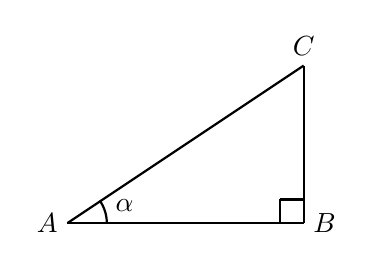
\begin{tikzpicture}[scale=1]
	\draw[-, thick, black] (0,0) -- (3,0);
	\draw[-, thick, black] (3,0) -- (3,2);
	\draw[-, thick, black] (3,2) -- (0,0);
	
	\node[black, left] at  (0,0) {$A$};
	\node[black, right] at  (3,0) {$B$};
	\node[black, above] at  (3,2) {$C$};
	% angle droit
	\draw[-, thick, black] (3,.3)-- (2.7,.3);
	\draw[-, thick, black] (2.7,.3)-- (2.7,0);
	
	% angle
	\draw [black,thick,domain=0:35] plot ({.5*cos(\x)}, {.5*sin(\x)})
	node[right, xshift=2, yshift=-2] {$\alpha$};
\end{tikzpicture}
\end{multicols}

		


\exemulticols{}{
	Calculer la longueur \textbf{exacte} de tous les côtés des triangles rectangles ci-contre.
	
	
%	Données : 
%	\begin{align*}
%		\sin(30^\circ) &= \cos(60^\circ) = \frac12, \\
%		\cos(30^\circ) &= \sin(60^\circ) = \frac{\sqrt{3}}2, \\
%		\tan(30^\circ) &= \frac1{\sqrt{3}}, \quad \tan(60^\circ) =\sqrt{3}.
%	\end{align*}
}{
	\null\vspace{-2cm}
	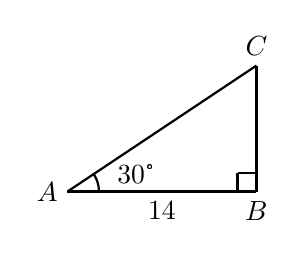
\begin{tikzpicture}[scale=.8]
		\draw[-, thick, black] (0,0) -- (3,0) node[midway, below] {$14$};
		\draw[-, thick, black] (3,0) -- (3,2);
		\draw[-, thick, black] (3,2) -- (0,0);
		
		\node[black, left] at  (0,0) {$A$};
		\node[black, below] at  (3,0) {$B$};
		\node[black, above] at  (3,2) {$C$};
		% angle droit
		\draw[-, thick, black] (3,.3)-- (2.7,.3);
		\draw[-, thick, black] (2.7,.3)-- (2.7,0);
		
		% angle
		\draw [black,thick,domain=0:35] plot ({.5*cos(\x)}, {.5*sin(\x)})
		node[right=5pt] {$30$°};
	\end{tikzpicture}
	\hfill
	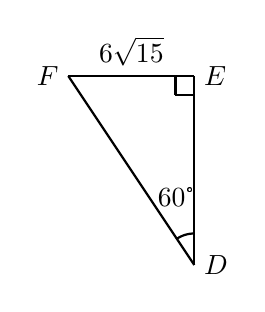
\begin{tikzpicture}[scale=.8, rotate=90]
		\draw[-, thick, black] (0,0) -- (3,0);
		\draw[-, thick, black] (3,0) -- (3,2)  node[midway, above] {$6\sqrt{15}$} ;
		\draw[-, thick, black] (3,2) -- (0,0);
		
		\node[black, right] at  (0,0) {$D$};
		\node[black, right] at  (3,0) {$E$};
		\node[black, left] at  (3,2) {$F$};
		% angle droit
		\draw[-, thick, black] (3,.3)-- (2.7,.3);
		\draw[-, thick, black] (2.7,.3)-- (2.7,0);
		
		% angle
		\draw [black,thick,domain=0:35] plot ({.5*cos(\x)}, {.5*sin(\x)})
		node[above=8pt] {$60$°};
	\end{tikzpicture}
} {exe:aut1}{}

\exe{}{
	Calculer $\cos^2(\theta) + \sin^2(\theta)$ pour $\theta = 30^\circ$ et $\theta =60^\circ$.
}{exe:c2s2-vérif}{
	TODO
}

\exe{}{
	Vérifier qu'on a bien $\tan(\theta) = \dfrac{\sin(\theta)}{\cos(\theta)}$ pour $\theta = 30^\circ$ et $\theta =60^\circ$.
}{exe:tan-vérif}{
	TODO
}

\subsection*{Projeté orthogonal}


\exemulticols{}{
	Un homme souhaite traverser une rivière en passant le moins de temps possible dans l'eau.
	%Celui-ci part du point vert et dois arriver au point rouge.
	
	En supposant qu'il avance à vitesse constante dans l'eau, quel est le chemin idéal qu'il doit prendre ?
	\vfill\null
}{
	\null\vspace{-50pt}
	\begin{center}
	\begin{tikzpicture}[scale=.8]
		\begin{axis}[xmin = 0, xmax=8, ymin=-.5, ymax=1.1,
		axis x line=none, axis y line=none, 
		grid=none,
		]
			\begin{scope}
			\clip[rotate=15] (axis cs:0,-.4) rectangle (axis cs:10,.4);
			\foreach \i in {-3, -2, -1, ..., 3}
				\addplot[no marks, BLUE_E, -, thick, rotate=15] expression[domain=0:10, samples=200]{cos(x*180*1.3)/8+\i/8};
			\end{scope}
			
			\draw[very thick, YELLOW_E, rotate=15] (axis cs:0,-.4) rectangle (axis cs:10,.4);
				
			\addplot[mark=*, mark size=2pt, GREEN_E] (2,-.27) node[below=3pt]{Départ};
			\addplot[mark=*, mark size=2pt, RED_E] (6,.82) node[above=3pt]{Arrivée};
		\end{axis}
	\end{tikzpicture}
	\end{center}
}{exe:riviere}{
	TODO
}


\begin{multicols}{2}
	\begin{center}
	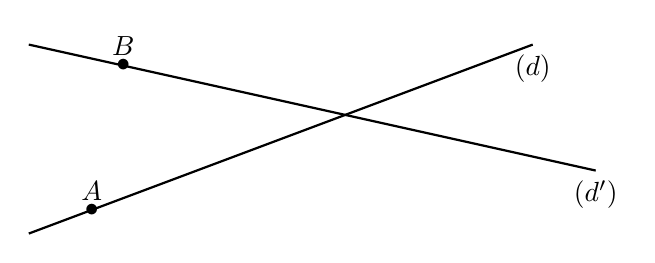
\begin{tikzpicture}[scale=.8]
		\draw[-, thick, black] (0,0) -- (8, 3) node[below]{$(d)$};
		\draw[-, thick, black] (0,3) -- (9, 1) node[below]{$(d')$};
	
		\node[black] at (1, 3/8) {$\bullet$};
		\node[black, above] at (1, 3/8) {$A$};
		
		\node[black] at (1.5, 24/9) {$\bullet$};
		\node[black, above] at  (1.5, 24/9) {$B$};
	\end{tikzpicture}
	\end{center}
	
\exe{}{
	Dans la figure ci-dessous, tracer un point $C$ tel que $A$ soit le projeté orthogonal de $C$ sur $(d)$ et que $B$ soit le projeté orthogonal de $C$ sur $(d')$.
} {exe:proj2}{}
\end{multicols}

\exe{}{
	Tracer une droite quelconque et un point n'appartenant pas à cette droite.
	À l'aide uniquement d'un compas, tracer le projeté orthogonal du point sur la droite.
} {exe:projperp-compas}{}

\exemulticols{}{
	Dans la figure ci-dessous, tracer
		\begin{enumerate}
			\item le point $B$, projeté orthogonal de $A$ sur $(d')$ ;
			\item le point $C$, projeté orthogonal de $B$ sur $(d)$ ;% et
			\item le point $D$, projeté orthogonal de $C$ sur $(d')$.
		\end{enumerate}
		
	Que dire des droites $(AB)$ et $(CD)$ ? Justifier.
}{
	\begin{center}
	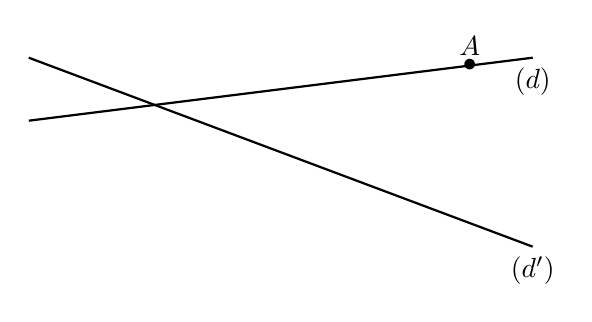
\begin{tikzpicture}[scale=.8]
		\draw[-, thick, black] (0,0) -- (8, 1) node[below]{$(d)$};
		\draw[-, thick, black] (0,1) -- (8, -2) node[below]{$(d')$};
	
		\node[black] at (7, 7/8) {$\bullet$};
		\node[black, above] at  (7, 7/8)  {$A$};
	\end{tikzpicture}
	\end{center}
} {exe:projpara}{}

%\exemulticols{}{
%	Un homme est dans une salle pentagonale comme schématisé ci-dessous.
%	Celui-ci souhaite toucher les murs $[AB], [CD], [AE], [BC],$ et $[ED]$ dans cet ordre en effectuant le trajet le plus court à chaque déplacement.
%	Tracer ses déplacements sur la figure si son point de départ est le point $M$.
%}{
%	\begin{center}
%	\begin{tikzpicture}
%		\draw[-, thick, black] (0,0) node{$\bullet$} -- (2.8, -1.2) node{$\bullet$};
%		\draw[-, thick, black] (2.8,-1.2) node{$\bullet$} -- (4, 1.5) node{$\bullet$};
%		\draw[-, thick, black] (4, 1.5) node{$\bullet$} -- (1.95,3) node{$\bullet$};
%		\draw[-, thick, black] (1.95,3) node{$\bullet$} -- (.3,2.3)  node{$\bullet$};
%		\draw[-, thick, black] (.3,2.3) node{$\bullet$} -- (0,0) node{$\bullet$};
%		
%		\node[black, below] at  (0,0)  {$A$};
%		\node[black, right] at  (2.8,-1.2)  {$B$};
%		\node[black, right] at  (4, 1.5)  {$C$};
%		\node[black, above] at  (1.95,3)  {$D$};
%		\node[black, left] at (.3,2.3)  {$E$};
%		
%		
%		\node[black, above] at (1.2, 1) {$M$};
%		\node[black] at (1.2, 1) {$\times$};
%	
%	\end{tikzpicture}
%	\end{center}
%} {exe:pentaperp}{}


\exe{}{
	On considère une droite $(d)$ et les points $A$ et $B$ distincts n'appartenant pas à la droite $(d)$.
	On note $A'$ et $B'$ les projetés orthogonaux respectifs des points $A$ et $B$ sur la droite $(d)$.
	
	Calculer la longueur $AB$ sachant que $AA' =1, BB' = 5$, et $A'B' = 4$. 
	Distinguer deux cas selon que les points sont ou non du même côté de $(d)$.
} {exe:dist-lift}{}

\subsection*{Hauteurs et aires}



\exemulticols{}{
	Considérons le triangle $ABC$ d'aire $\text{Aire}(ABC) = \frac{3}{10}$ et tel que $AB=\frac34$ et $CD =\frac25$.
	
	Est-ce que les droites $(AB)$ et $(CD)$ sont perpendiculaires ? Justifier.
	\vfill\,
}{
	\begin{center}
	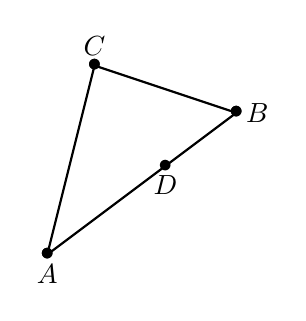
\begin{tikzpicture}[scale=.6]
		\draw[-, thick, black] (0,0) node{$\bullet$} -- (4, 3) node{$\bullet$};
		\draw[-, thick, black] (4, 3) node{$\bullet$} -- (1,4) node{$\bullet$};
		\draw[-, thick, black] (1,4) node{$\bullet$} -- (0,0) node{$\bullet$};
		
		\node[black, below] at  (0,0)  {$A$};
		\node[black, right] at  (4, 3)  {$B$};
		\node[black, above] at  (1,4) {$C$};
		
		
		\node[black] at  (2.5,2.5*3/4) {$\bullet$};
		\node[black, below] at  (2.5,2.5*3/4) {$D$};
	
	\end{tikzpicture}
	\end{center}
} {exe:aire-to-perp}{}


\exe{}{
	Considérons le triangle $ABC$ comme à l'exercice \ref{exe:aire-to-perp} et d'aire $\text{Aire}(ABC) = 8$ et tel que $AB=4$ et $AC =5$.
	Quelle longueur $AD$ doit-on choisir pour que les droites $(AB)$ et $(DC)$ soient perpendiculaires ?
} {exe:perp-to-aire}{}


\exemulticols{}{
	Soit $ABC$ le  triangle rectangle ci-contre, avec $BH$ une de ses hauteurs.
	\begin{enumerate}[label=\alph*.]
		\item Calculer $AB$.
		\item Calculer l'aire du triangle $ABC$.
		\item En déduire $BH$.
	\end{enumerate}
}{
	\begin{center}
	\usetikzlibrary{calc}
	\begin{tikzpicture}[scale=1]
	
	% triangle
	\draw[-, very thick] (0,0) coordinate (A) node[left]{$A$}
		-- (4, .5) coordinate (C) node[right]{$C$}
		-- (1,2) coordinate (B) node[above]{$B$}
		-- cycle;
	
	\draw[- , thick, decorate, decoration = {brace, mirror, raise=3pt}] (A) -- (C) node[midway,below=5pt,rotate=7]{104};
	\draw[- , thick] (B)--(C) node[midway,above,rotate=-26]{\underline{96}};
	
	%hauteur
	\draw[-, very thick, BLUE_E] (B) -- (80/65, 10/65) coordinate (H) node[above left] {$H$}; 
	
	% angles droits
	\draw[-, thick, RED_E] ($(H)+.07*(C)$) -- ($(H)+.07*(C) + .15*(B)-.15*(H)$) -- ($(H) + .15*(B)-.15*(H)$) ;
	
	\draw[-, thick, RED_E] ($(B) + .08*(C) - .08*(B)$) -- ($(B) + .08*(C) - .08*(B) - .12*(B)$) -- ($(B) - .12*(B)$) ;
	
	\end{tikzpicture}
	\end{center}
}{exe:aire-hauteur}{
	TODO
}


\begin{multicols}{2}

	\begin{center}
	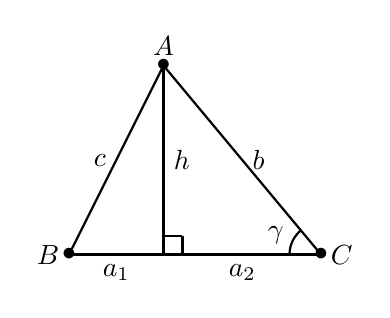
\begin{tikzpicture}[scale=.8]
		\draw[-, thick, black] (0,0) node{$\bullet$} -- (1.5,0) node[midway, below] {$a_1$};
		\draw[-, thick, black] (1.5,0) -- (4,0) node[midway, below] {$a_2$};
		\draw[-, thick, black] (4, 0) node{$\bullet$} -- (1.5,3) node[midway, right] {$b$};
		\draw[-, thick, black] (1.5,3) node{$\bullet$}-- (0,0) node[midway, left] {$c$};
		
		\node[black, left] at  (0,0) {$B$};
		\node[black, right] at  (4,0) {$C$};
		\node[black, above] at  (1.5,3) {$A$};
		
		\draw[-, thick, black] (1.5,0)-- (1.5,3) node[midway, right] {$h$};
		
		% angle droit
		\draw[-, thick, black] (1.5,.3)-- (1.8,.3);
		\draw[-, thick, black] (1.8,.3)-- (1.8,0);
		
		% angle
		\draw [black,thick,domain=130:180] plot ({4+.5*cos(\x)}, {.5*sin(\x)})
		node[left=5pt, above] {$\gamma$};
	\end{tikzpicture}
	\end{center}
	
\exe{, difficulty=1}{
	Soit un triangle $ABC$ quelconque représenté ci-contre. On pose $a=a_1 + a_2 = BC$.
	
	Montrer la \emph{formule de l'aire} 
		\[ \text{Aire}(ABC) = \dfrac12 ab \sin(\gamma). \]
	\vfill\,
}{exe:formule-aire}{
}
\end{multicols}

\subsection*{Trigonométrie}


%\exe{}{
%	En construisant un triangle équilatéral de côté 1, calculer les valeurs suivantes.
%		\begin{multicols}{2}
%		\begin{enumerate}
%			\item $\cos(60\degree)$
%			\item $\sin(30\degree)$
%			\item $\sin(60\degree)$
%			\item $\cos(30\degree)$
%			\item $\tan(30\degree)$
%			\item $\tan(60\degree)$
%		\end{enumerate}
%		\end{multicols}
%} {exe:cos-sin-tan-equi}{}



\begin{multicols}{2}
\exe{}{
	Dans la figure ci-dessous, calculer $x$ à l'aide du théorème de Pythagore, puis $y$ à l'aide du théorème de Thalès ou de la trigonométrie.
}{exe:pyth-thalès}{
	TODO $x = 3\sqrt2 - 1$ et $y=3 - \dfrac{\sqrt2}2$ je crois.
}
	\begin{center}
	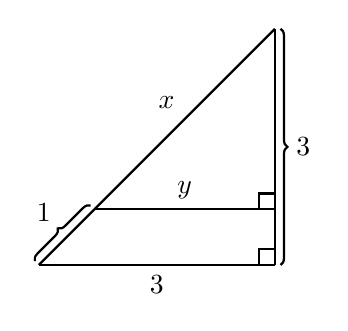
\begin{tikzpicture}[scale=1, rotate=0]
	\draw[-, thick] 
	(0,0) -- (3,0) node[midway, below] {$3$};
	\draw[-, thick] 
	(3,0) -- (3, 3);
	\draw[-, thick, decorate, decoration={brace, raise=2pt, mirror}] 
	(3,0) -- (3, 3) node[midway, right=4pt] {$3$};
	\draw[-, thick] 
	(0,0) -- (0.707, 0.707);
	\draw[-, thick, decorate, decoration={brace, raise=2pt}] 
	(0,0) -- (0.707, 0.707) node[midway, above left=2pt] {$1$};
	\draw[-, thick] 
	 (0.707, 0.707) -- (3,3) node[midway, above left] {$x$};
	\draw[-, thick] 
	 (0.707, 0.707) -- (3,.707) node[midway, above] {$y$};
	
	\draw[-, thick] (2.8,0) -- (2.8, .2) -- (3, .2);
	\draw[-, thick] (2.8,0.707) -- (2.8, .907) -- (3, .907);
	\end{tikzpicture}
	\end{center}
	\begin{center}
	\usetikzlibrary{angles, quotes} 
	\begin{tikzpicture}[scale=1, rotate=90]
	\draw[-, thick] 
	(0,0) coordinate (A) -- 
	(2.179,0) coordinate (B) -- 
	(2.179,3)  coordinate (C) node[midway, above] {$3$} -- 
	cycle node[midway, below left] {$z$} 
	pic ["36°", draw,-,BLUE_E,thick,angle radius=25pt, angle eccentricity=1.5] {angle = A--C--B};
	
	\draw[-, thick] (1.979,0) -- (1.979, .2) -- (2.179, .2);
	\end{tikzpicture}
	\end{center}

\exe{}{
	Dans la figure ci-dessus, calculer $z$ en sachant que $\cos(36^\circ) = \frac{1+\sqrt5}4$.
}{exe:cos36}{
	TODO
}
\end{multicols}



\exemulticols{}{
	Calculer la longueur \textbf{exacte} de tous les côtés des triangles rectangles suivants.
}{
	\null\vspace{-30pt}
	\centering
	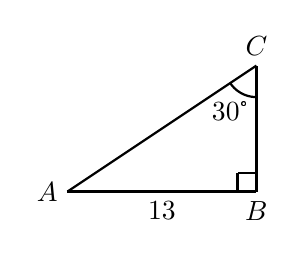
\begin{tikzpicture}[scale=.8]
		\draw[-, thick, black] (0,0) -- (3,0) node[midway, below] {$13$};
		\draw[-, thick, black] (3,0) -- (3,2);
		\draw[-, thick, black] (3,2) -- (0,0);
		
		\node[black, left] at  (0,0) {$A$};
		\node[black, below] at  (3,0) {$B$};
		\node[black, above] at  (3,2) {$C$};
		% angle droit
		\draw[-, thick, black] (3,.3)-- (2.7,.3);
		\draw[-, thick, black] (2.7,.3)-- (2.7,0);
		
		% angle
		\draw [black,thick,domain=215:270] plot ({3+.5*cos(\x)}, {2+.5*sin(\x)})
		node[below=5pt, left=-1pt] {$30$°};
	\end{tikzpicture}
	\hfill
	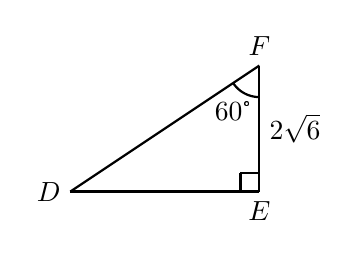
\begin{tikzpicture}[scale=.8, rotate=0]
		\draw[-, thick, black] (0,0) -- (3,0);
		\draw[-, thick, black] (3,0) -- (3,2) node[midway, right] {$2\sqrt{6}$} ;
		\draw[-, thick, black] (3,2) -- (0,0);
		
		\node[black, left] at  (0,0) {$D$};
		\node[black, below] at  (3,0) {$E$};
		\node[black, above] at  (3,2) {$F$};
		% angle droit
		\draw[-, thick, black] (3,.3)-- (2.7,.3);
		\draw[-, thick, black] (2.7,.3)-- (2.7,0);
		
		% angle
		\draw [black,thick,domain=215:270] plot ({3+.5*cos(\x)}, {2+.5*sin(\x)})
		node[below=5pt, left=-1pt] {$60$°};
	\end{tikzpicture}
} {exe:aut2}{}




%\exe{}{
%
%	\begin{multicols}{2}
%	\begin{center}
%	%
\includegraphics[scale=.75]{14p141.png}
%	\, \,
%	%
\includegraphics[scale=.6]{15p141.png}
%	\end{center}
%	\end{multicols}
%} {exe:dunno2}{}

\exe{, difficulty=1}{
	En étant donné que 
		\begin{align*}
			\sin(15\degree) = \dfrac{\sqrt{6}-\sqrt{2}}4 && \text{ et } && \cos(36\degree) = \dfrac{1+\sqrt{5}}4,
		\end{align*}
	vérifier que $\cos(15\degree) = \frac{\sqrt{6}+\sqrt{2}}4$ et donner la valeur \textbf{exacte} de $\sin(36\degree)$.
} {exe:c2-s2-1}{}

%\exe{
%	Sur un terrain, un footballer se trouve à $16,50$ mètres de la ligne de but et à $25$ mètres du poteau de but le plus proche. La largeur des cages est de $7,32$ mètres.
%	
%	Déterminer l'angle de tir $\theta$ en arrondissant au degré près.
%}
%{}


\exemulticols{, difficulty=1}{
	On considère un point $P$ sur un quart de cercle de rayon $2$ et de centre $O$, l'origine d'un repère.
	On pose $\theta \in [0; 90\degree]$ l'angle entre la droite $(OP)$ et l'axe des abscisses.
	Chaque choix de $\theta$ correspond donc à un point et aussi à un triangle comme représentés ci-dessous.
	
	\begin{enumerate}
		\item
		Montrer que l'aire $f(\theta)$ du triangle est donnée par 
			\[ f(\theta) = 2 \cos(\theta) \sin(\theta). \]
		\item
		Grapher $\C_f$ et en déduire l'angle maximisant $f$ ainsi que les coordonnées du point $P$ correspondant.
	\end{enumerate}
}{
	\begin{center}
	\begin{tikzpicture}[>=stealth, scale=1]
		\begin{axis}[xmin = 0, xmax=2.1, ymin=0, ymax=2.1, axis x line=middle, axis y line=middle, axis line style=->, grid=both, grid style = {opacity=.5}]
			\addplot[no marks, BLUE_E, -, very thick] expression[domain=0:2, samples=101]{sqrt(4-x^2)};
			\addplot[mark=*, mark size = 1, black, thick] (0.625*2, 0.7805*2) node[right=3pt] {$P({\color{PURPLE}x};{\color{RED_E}y})$};
			
			
			\addplot[black, dashed, very thick] expression[domain=0:0.625*2, samples=2]{0.7805/0.625*x}
			node[midway, above=]{$2$};
			
			\addplot[no marks, GREEN_E, -, very thick] expression[domain=0.11:0.1732, samples=101]{sqrt(.03-x^2)}
			node[right, pos=.3] {$\theta$};
			
			\draw[black, dashed, very thick] (axis cs:0.625*2, 0) -- (axis cs:0.625*2,0.7805*2);
			
			% angle droit
			\draw[-, thick, black] (axis cs:0.585*2,0) -- (axis cs:0.585*2,.05*2) -- (axis cs:0.625*2,.05*2);
		\end{axis}
	\end{tikzpicture}
	\end{center}
} {exe:opt-area}{}


\subsection*{Approfondissements}



\exe{, difficulty=2}{
	On souhaite démontrer le \emphindex{théorème d'Al-Kashi}\footnotemark, ou \emphindex{loi des cosinus}, généralisant le théorème de Pythagore aux triangles non nécessairement rectangles.
	Reconsidérons donc le triangle $ABC$ de l'exercice \ref{exe:formule-aire}.
	
	\begin{enumerate}
		\item Montrer d'abord que $a_2 = b \cos(\gamma)$.
			%\begin{align*} h = b \sin(\gamma), && \text{ et } && a_2 = b \cos(\gamma). \end{align*}
		\item
		Donner les identités de Pythagore dans les deux triangles rectangles $HAC$ et $BAH$, où $H$ est le projeté orthogonal de $A$ sur $(BC)$.
		\item
		Utiliser $a_1 = a - a_2$ et les expressions obtenues pour conclure que
			\[ c^2 = a^2 + b^2 - 2ab \cos(\gamma). \]
	\end{enumerate}
}{exe:al-kashi}{
	Posons $H$ le projeté orthogonal de $A$ sur $(BC)$.
	\begin{enumerate}
		\item 
			Le résultat est obtenu par trigonométrie dans le triangle rectangle $HAC$.
		\item
		On obtient
			\begin{align*}
				c^2 &= h^2 + a_1^2, \\
				b^2 &= h^2 + a_2^2. 
			\end{align*}
		\item
		En partant de la gauche on a 
			\begin{align*}
				c^2 &= h^2 + a_1^2, \\
					&= h^2 + (a-a_2)^2, \\
					&= h^2 + a_2^2 + a^2 - 2aa_2, \\
					&= b^2 + a^2 - 2ab\cos(\gamma),
			\end{align*}
		comme requis.
	\end{enumerate}
}

\footnotetext{Ghiyath ad-Din Jamshid Mas`ud al-Kashi (1380? - 1429), mathématicien et astronome perse.}

\exe{, difficulty=1}{
	Soit un triangle aux angles $\alpha, \beta, \gamma$ opposés au côtés de longueur $a, b, c$ respectivement.
	En considérant d'abord la hauteur $h$ partageant l'angle $\gamma$, montrer que $h = a\sin\beta = b\sin\alpha$.
	
	En déduire la \emphindex{loi des sinus} :
		\[ \dfrac{a}{\sin\alpha} = \dfrac{b}{\sin\beta} = \dfrac{c}{\sin\gamma}. \]
}{exe:loi-sinus}{
	TODO
}

\exe{, difficulty=2}{
	En musique, la gamme classique contient douze notes avec un rapport de fréquence de 2 sur l'octave.
	La gamme est dite à tempérament égal si le rapport de fréquence entre deux notes consécutives est toujours le même.
	Notons ce rapport $r\in\R$.
	Justifier que $r^{12} = 2$ puis démontrer que $r$ est un nombre irrationnel : $r \not\in\Q$.
}{exe:temp-égal}{
	Le rapport de fréquence entre deux notes consécutives étant toujours $r$, on multiplie $r$ par lui-même 12 fois pour obtenir le rapport de fréquence entre deux notes de distance $12$, c'est-à-dire deux notes séparée par un octave.
	Ainsi $r^{12} = 2$ car l'octave correspond à un rapport de fréquence de 2.
	
	Supposons désormais que $r$ soit rationnel. Alors $r^{6}$ est aussi rationnel.
	Cependant, $(r^6)^2 = r^{12} = 2$, donc $r^{6} = \sqrt2$, qui n'est pas rationnel. \Large\Lightning
}

\exe{, difficulty=1}{
	Montrer que $\sqrt2 = 1 + \frac1{1+\sqrt2}$.
	En déduire que $\sqrt2 = 1 + \frac1{2 + \frac1{1+\sqrt2}}$ et que
		\[\sqrt2 = 1 + \cfrac1{2 + \cfrac1{2 + \cfrac1{2 + \cfrac1{1+\sqrt2}}}}. \]
	Exprimer le rationnel $1 + \frac1{2 + \frac1{2 + \frac12}}$ sous la form $\frac{p}{q}$ avec $p$ et $q$ premiers entre eux et calculer $\left| \sqrt2 - \frac{p}q \right|$ au millième près.
	Faire idem avec $1 + \frac1{2 + \frac1{2 + \frac1{2 + \frac12}}}$.
}{exe:frac-continue-sqrt2}{
	En manipulant l'équation on se retrouve à vouloir montrer que $\sqrt2 - 1 = \dfrac1{\sqrt2+1}$, ce qui est équivalent à $(\sqrt2 - 1)(\sqrt2 + 1) = 1$, vrai par identité remarquable (ou par distributivité simple).
	
	Comme $\sqrt2 = 1 + \dfrac1{1+\sqrt2}$, on peut remplacer le $\sqrt2$ dans l'expression de droite par toute l'expression de droite.
	On obtient donc $\sqrt2 = 1 + \cfrac1{1 + 1 + \cfrac1{1+\sqrt2}} = 1 + \cfrac1{2 + \cfrac1{1+\sqrt2}}$ comme voulu.
	On obtient l'expression d'après en répétant le même raisonnement.
	
	Par simplifications simples, on trouve $\dfrac{p}{q} = \dfrac{17}{12}$.
	La calculatrice nous donne alors $\left| \sqrt2 - \dfrac{17}{12} \right| \approx 0,002$.
	
	Finalement, remarquons que 
	\begin{align*}
		1 + \cfrac1{2 + \cfrac1{2 + \cfrac1{2 + \cfrac12}}} &= 1 + \cfrac1{1+ 1 + \cfrac1{2 + \cfrac1{2 + \cfrac12}}}, \\
			&= 1 + \cfrac1{1+ \dfrac{17}{12}} = \dfrac{41}{29}.
	\end{align*}
	Le rationnel $\dfrac{41}{29}$ vérifie $\left| \sqrt2 - \dfrac{41}{29} \right| \approx 0,0004$, soit 5 fois plus proche de $\sqrt2$ que $\dfrac{17}{12}$ l'est.
}


\exe{, difficulty=3}{
	Posons $\Qsqrt{5} = \bigset{ r + s \sqrt5 \tq r, s \in \Q} \subseteq \R$ et considérons $x = r + s\sqrt5$ et $y=p+q\sqrt5$ avec $r, s, p, q \in\Q$.
	\begin{enumerate}
		\item
		Montrer que $\Q \subseteq \Qsqrt5$ est une inclusion stricte.
		\item
		Montrer que $x=y \iff r = p \et s = q$.
	\end{enumerate}
	Considérons désormais la fonction « conjugué » $f$ définie par $f\bigl(r + s\sqrt5\bigr) = r - s\sqrt5$.
	\begin{enumerate}[resume]
		\item
		Montrer que $f(x+y) = f(x)+f(y)$ et que $f(xy) = f(x)f(y)$.
		\item
		Montrer que si $f(x) = x$, alors $x\in\Q$.
		\item
		Conclure à l'aide des deux dernières questions que
			\[ \dfrac1{2^{256}\sqrt5}\left[ \left({1+\sqrt5}\right)^{256} - \left({1-\sqrt5}\right)^{256}\right] \]
		est un nombre rationnel.
		(C'est en fait un nombre entier et le terme $256$ de la suite de Fibonacci)
		\item
		Montrer que $\Qsqrt{5} \neq \R$ en montrant que $\sqrt2 \not\in \Qsqrt{5}$.
	\end{enumerate}
} {exe:Qsqrt2}{
	À rendre pour possibilité de points bonus à la prochaine évaluation.
	Ni correction ni points ne seront attribués à un travail suspect ou ne démontrant pas une bonne compréhension de l'exercice.
	
	Indication pour la question 2 : il est possible de montrer en premier lieu que $x = 0 \iff r=s=0$.
	On dit alors que $1$ et $\sqrt5$ sont \emph{linéairement indépendants} sur $\Q$.
	
	Indication pour la question 5 : appliquer $f$ à la quantité $\left({1+\sqrt5}\right)^{256} - \left({1-\sqrt5}\right)^{256}$ et conclure qu'elle est égale à $s\sqrt5$ pour un $s\in\Q$ rationnel.
	
	\underline{Discussion}
	
	L'exercice fait l'étude du corps d'extension des nombres rationnels auxquels on a ajouté la racine carrée de 5.
	Il suit de la question 6 que l'ensemble 
		\[ \Q\bigl(\sqrt2, \sqrt5\bigr) = \bigset{ r + s \sqrt2 + t\sqrt5 \tq r, s, t \in \Q} \]
	est un sur-ensemble strict de $\Qsqrt5$ qui n'est toujours pas égal à $\R$.
	
	La {théorie de Galois}\footnotemark généralise ces exemples et permet notamment de répondre par la négative aux trois grands problèmes de l'Antiquité : la duplication du cube, la trisection de l'angle, et la quadrature du cercle.
	\footnotetext{Évariste Galois (1811-1832), mathématicien français mort à l'âge de 20 ans. }
	Essentiellement, chaque construction à la règle et au compas à partir d'un repère orthonormé ajoute la racine carrée d'un nombre déjà constructible jusqu'ici.
	La racine carrée de 2 est par exemple constructible grâce au théorème de Pythagore comme distance entre $(1 ; 0)$ et $(0;1)$.
	En montrant que certains nombres ne peuvent pas appartenir à de telles extensions, on démontre immédiatement qu'ils sont non constructibles.
}





%%%%%%%%%%%

\newpage
\fancyhead[C]{\textbf{Solutions}}
\shipoutAnswer

\end{document}
